\section{Max-Input Head-to-Head}

\begin{frame}{10000x10000 Stress Test: Runtime and Comparison Outcomes}
\centering
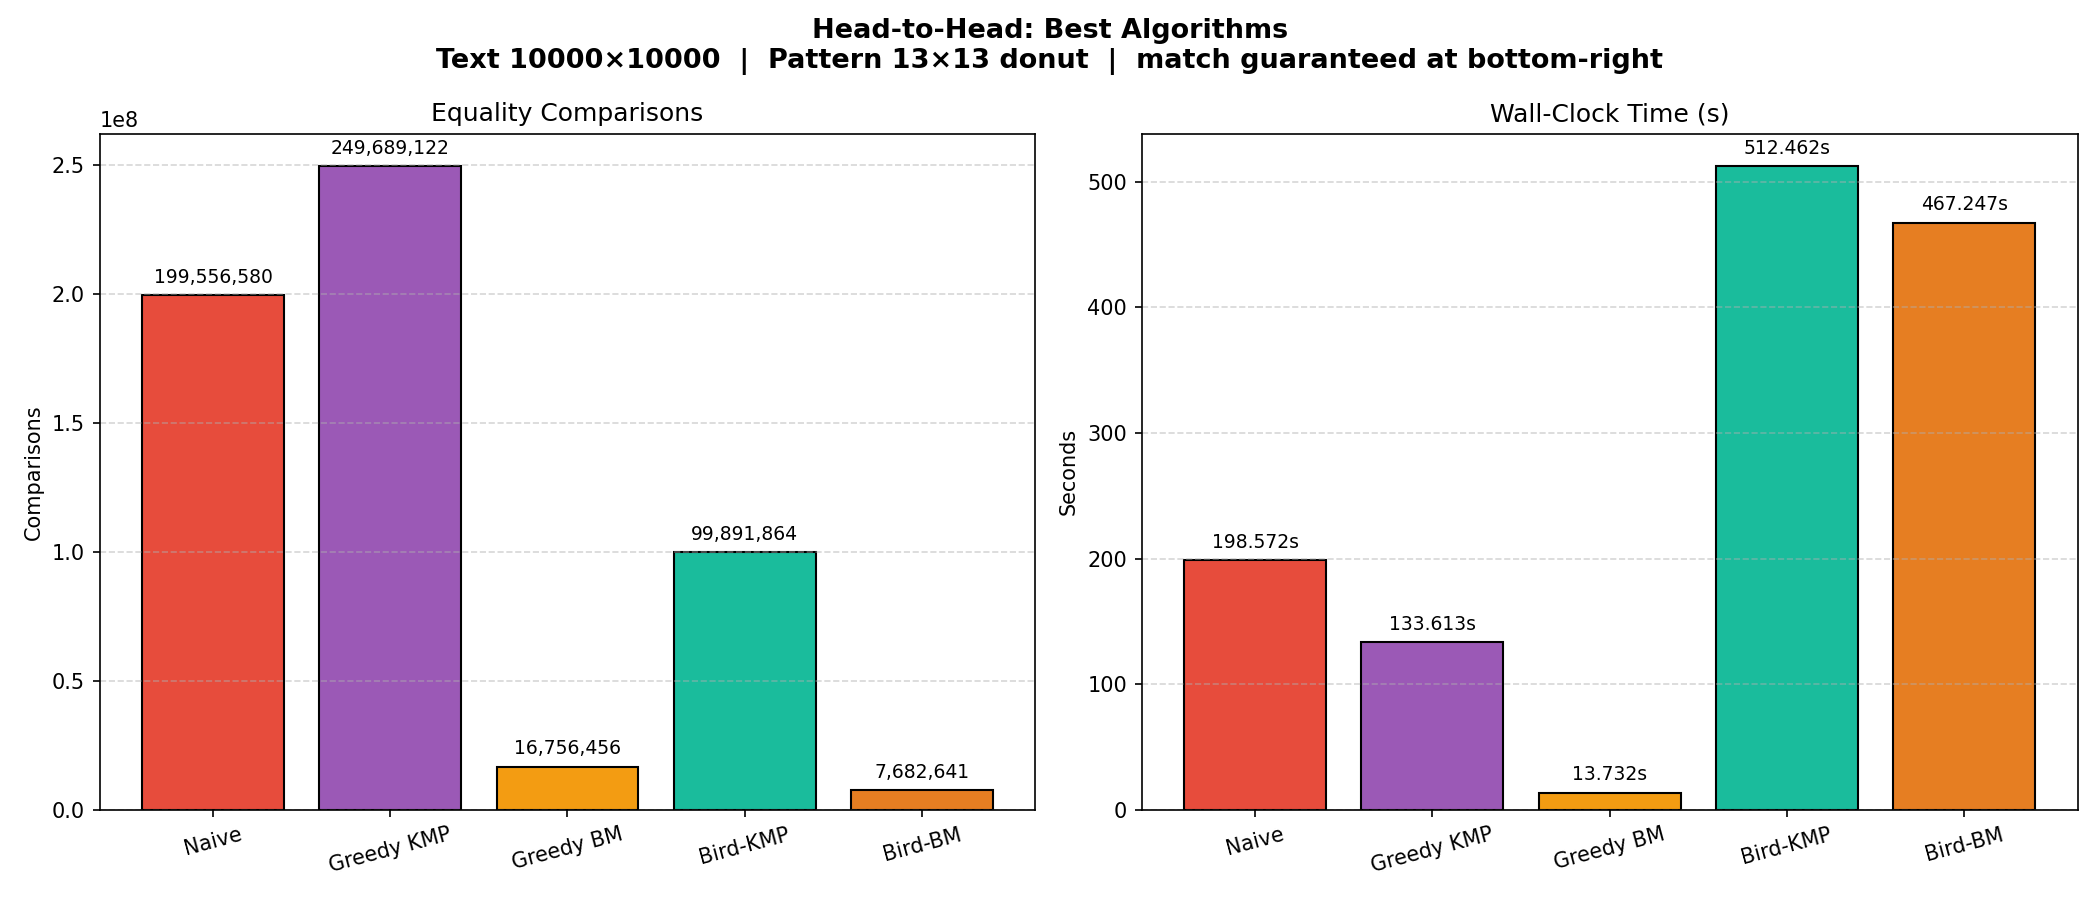
\includegraphics[width=\linewidth,height=0.53\textheight,keepaspectratio]{head_to_head.png}

\vspace{0.3em}
\keymsg{Fastest runtime: \HeadBestTimeAlgo{} at \HeadBestTimeValue{} s; best speedup vs Naive: \HeadBestSpeedupValue{}x.}
\sourcenote{\texttt{results\_head\_to\_head.csv} and \texttt{head\_to\_head.png}}
\end{frame}

\begin{frame}{Why Bird-BM Can Win Comparisons but Lose Runtime}
\small
\begin{itemize}
  \item In this implementation, Bird-family preprocessing and traversal overhead is significant.
  \item The stress test magnifies constant-factor costs over huge matrices.
  \item Result: Bird-BM has lowest comparisons (\HeadCompBirdBM{}) but much higher runtime (\HeadTimeBirdBM{} s).
  \item Greedy BM is a better practical runtime choice here (\HeadTimeGreedyBM{} s).
\end{itemize}
\begin{block}{Engineering implication}
Implementation detail dominates at scale; comparison-optimal is not automatically throughput-optimal.
\end{block}
\end{frame}
